% ====================================================================
% JMP_seminar_deck_v1.tex
%   Unequal Job Opportunities and the Measurement of Welfare Inequality
%   Seminar deck, built from the FROZEN content document
%     manuscript/JMP_seminar_deck_content_v1.md   (Goal-1 R-256)
%   against the frozen figure and table set at JMP commit b1dea12.
%
% Nothing here is science.  Every number is a macro from
%   beamer/deck_numbers_v1.tex, generated by beamer/make_deck_macros_v1.py
% from the named seminar-sprint artefacts; no number is typed by hand.
% Every figure is a PDF from beamer/figures/, copied from the frozen
% sprint figure set.
%
% Preamble, theme, colours and note-page template are shared with the
% companion theory talk via beamer/jmp_beamer_preamble.tex.
%
% ---- BUILDS ---------------------------------------------------------
%   45-minute (default)  ./build_deck_v1.sh
%   25-minute            ./build_deck_v1.sh short      (\def\ShortDeck{})
%   rehearsal (notes)    ./build_deck_v1.sh rehearsal  (\def\RehearsalDeck{})
%   all three            ./build_deck_v1.sh all
%
% ---- TIMING BUDGET (45-minute slot; 41.0 min of content) ------------
%   Part I   -- the question .............. slides  1-5    8.0 min
%   Part II  -- how it is estimated ....... slides  6-9    8.0 min
%   Part III -- what the model fits ....... slides 10-13   7.0 min
%   Part IV  -- what it finds ............. slides 14-21  15.5 min
%   Part V   -- close ..................... slides 22-23   2.5 min
%   ------------------------------------------------------------------
%   TOTAL ................................. 23 slides    41.0 min
%   plus 4 backup slides, not in the running order.
% ====================================================================
\documentclass[10pt]{beamer}

% ====================================================================
% jmp_beamer_preamble.tex --- shared preamble for the JMP seminar deck.
%
% REUSED VERBATIM from the companion theory talk
%   beamer/reference/Theory_talk/slides/Presentation.tex
%     "Jobs and Well-Being Measurement" (Haydar and Maniquet)
% so that the two decks read as one visual family.  The elements carried
% over unchanged are marked [THEORY-TALK] below; everything else is an
% addition this deck needs and the theory talk does not.
%
% Consistency is the point: same class options, same theme, same accent
% colour, same frame numbering, same appendix handling, same visible-link
% convention, same note-page template, same two-agent sketch palette.
% ====================================================================

% ---- [THEORY-TALK] class, theme and the deep-red accent -------------
\usetheme{metropolis}
\definecolor{deepred}{RGB}{150,25,35}
\setbeamercolor{frametitle}{bg=deepred}
\setbeamertemplate{navigation symbols}{}
% metropolis-defined accents (safe: these beamercolors exist in metropolis)
\setbeamercolor{progress bar}{fg=deepred}
\setbeamercolor{title separator}{fg=deepred}
% frame number as current/total, in deep red
\metroset{numbering=fraction}
\setbeamercolor{footline}{fg=deepred}
% backup appendix: keep the main frame total at the running-order count
\usepackage{appendixnumberbeamer}
% VISIBLE link colours for rehearsal (internal hyperlinks in deep red)
\hypersetup{colorlinks=true,linkcolor=deepred,citecolor=deepred,urlcolor=deepred}

% ---- [THEORY-TALK] encoding, language, maths, tables, tikz ----------
\usepackage[utf8]{inputenc}
\usepackage[english]{babel}
\usepackage{amsmath}
\usepackage{amssymb}
\usepackage{amsfonts}
\usepackage{booktabs}
\usepackage[official]{eurosym}   % \euro --- this deck quotes euro magnitudes
\usepackage{tikz}
\usetikzlibrary{decorations.pathreplacing,arrows.meta,positioning,fit,backgrounds}

% ---- [THEORY-TALK] the two-agent sketch palette --------------------
% red = agent i / household A ; blue = agent h / household B
\definecolor{agenti}{RGB}{200,30,40}
\definecolor{agenth}{RGB}{20,80,200}

% ---- [THEORY-TALK] notes on a second screen (rehearsal view) -------
% The rehearsal build turns this on; the projection build leaves it off.
\usepackage{pgfpages}
% Long notes overflow the note column by default; render them smaller,
% ragged-right, with tight paragraph spacing so the full text stays
% legible and inside the frame on the second screen.
%
% This deck's notes are longer than the theory talk's -- several run past
% one note page at \scriptsize and produced overfull \vbox warnings.  The
% template below keeps the theory talk's look and adds two things it
% needs: \tiny with a tighter baseline, and an \allowbreak-friendly
% vertical box so a long note breaks across note pages instead of
% overflowing.  Hyphenation is relaxed so no line runs into the margin.
\setbeamertemplate{note page}{%
  \vspace{0.3em}\par
  {\tiny\setlength{\parskip}{0.45em}\setlength{\parindent}{0pt}%
   \setlength{\emergencystretch}{3em}%
   \linespread{1.05}\selectfont
   \raggedright\insertnote\par}%
}
% Notes are prose, not code: let TeX hyphenate freely rather than push a
% long word past the measure.
\hyphenpenalty=50
\tolerance=2000

\DeclareMathOperator*{\argmax}{arg\,max}

% ====================================================================
% ADDITIONS for this deck (not in the theory talk)
% ====================================================================

% ---- channel colours ------------------------------------------------
% One colour per decomposition channel, used consistently on every slide
% that names a channel.  Preferences take the theory talk's agent-red so
% the two decks agree on which side of the argument is which.
\definecolor{chpref}{RGB}{200,30,40}     % preferences   (= agenti)
\definecolor{chacc}{RGB}{20,80,200}      % job access    (= agenth)
\definecolor{chearn}{RGB}{200,120,20}    % earning opportunities
\definecolor{chneeds}{RGB}{40,120,70}    % endowments and needs
\definecolor{chenv}{RGB}{60,60,70}       % the whole environment

% ---- the paper's notation ------------------------------------------
% Audience-facing channel names are WORDS on the slides; these commands
% exist so the words are spelled the same way every time they appear.
\newcommand{\pref}{\textcolor{chpref}{preferences}}
\newcommand{\Pref}{\textcolor{chpref}{Preferences}}
\newcommand{\acc}{\textcolor{chacc}{job access}}
\newcommand{\Acc}{\textcolor{chacc}{Job access}}
\newcommand{\earn}{\textcolor{chearn}{earning opportunities}}
\newcommand{\Earn}{\textcolor{chearn}{Earning opportunities}}
\newcommand{\needs}{\textcolor{chneeds}{household endowments and needs}}
\newcommand{\Needs}{\textcolor{chneeds}{Household endowments and needs}}
\newcommand{\env}{\textcolor{chenv}{the environment}}
\newcommand{\Env}{\textcolor{chenv}{The environment}}

% Symbols.  The theory-paper symbols W, z, R, A, y appear ONLY where the
% companion paper is cited; the estimation notation is separate.
\newcommand{\Wmeasure}{W}                      % theory-paper measure
\newcommand{\Jset}{\mathcal{J}}                % theory-paper job space
\newcommand{\Wone}{W^{1}}                      % theory-paper W^1
\newcommand{\yref}{\mathbf{y}^{w}}             % theory-paper reference pay
\newcommand{\gopp}{g}                          % estimated offer density
\newcommand{\uutil}{u}                         % preference index
\newcommand{\Wmm}{\mathrm{W}}                  % money-metric welfare level

% ---- headline / caveat call-outs -----------------------------------
\newcommand{\headline}[1]{{\large\textcolor{deepred}{#1}}}
\newcommand{\caveat}[1]{{\footnotesize\textcolor{deepred}{#1}}}
% a number with its numerical-integration band
\newcommand{\wband}[2]{#1\,\ensuremath{\pm}\,#2}

% ---- the 25-minute variant ------------------------------------------
% Every frame carries \shortdeck (in the 25-minute running order) or
% \longdeck (45-minute only).  \DeckShort, set by the driver file, drops
% the \longdeck frames; the default keeps everything.
%
% The frozen plan's 25-minute running order is 16 slides, reached from the
% 23 by FIVE cuts and TWO merges:
%   CUT   -> backup : 9, 12, 17, 18, 22          (\longdeck)
%   MERGE           : 6+7 -> one slide, 10+11 -> one slide
% So three tags, not two.  A merged pair is written as two full frames for
% the 45-minute deck; in the short deck the SECOND of the pair drops and
% the first shows its merged content.  23 - 5 - 2 = 16.
%
% Usage:  \shortdeck{\begin{frame}...\end{frame}}     kept in both
%         \longdeck{\begin{frame}...\end{frame}}      45-minute only (cut)
%         \mergedaway{\begin{frame}...\end{frame}}    45-minute only (merged)
%         \ifDeckShort ... \else ... \fi              inline merged content
\newif\ifDeckShort\DeckShortfalse
\newcommand{\shortdeck}[1]{#1}                       % always kept
\newcommand{\longdeck}[1]{\ifDeckShort\else#1\fi}    % cut to backup at 25 min
\newcommand{\mergedaway}[1]{\ifDeckShort\else#1\fi}  % folded into the previous
% content shown only in the merged (25-minute) form of a slide
\newcommand{\mergedonly}[1]{\ifDeckShort#1\fi}

% ---- figure helper ---------------------------------------------------
% Every figure is a PDF from the frozen sprint set, included by name from
% beamer/figures/.  \deckfig{name}{width fraction} keeps the call sites
% uniform and makes a missing file fail loudly at compile time.
\graphicspath{{figures/}}
% Heights leave room for the frametitle, the one caption line every figure
% slide carries, and the metropolis footline -- a taller box overflows the
% frame and shows up as an overfull \vbox.
\newcommand{\deckfig}[2]{%
  \begin{center}\includegraphics[width=#2\textwidth,height=0.70\textheight,%
    keepaspectratio]{#1}\end{center}}
\newcommand{\deckfigtwo}[4]{%
  \begin{columns}[c,onlytextwidth]
  \column{0.49\textwidth}\includegraphics[width=\textwidth,height=0.60\textheight,%
    keepaspectratio]{#1}\\{\centering\scriptsize #2\par}
  \column{0.49\textwidth}\includegraphics[width=\textwidth,height=0.60\textheight,%
    keepaspectratio]{#3}\\{\centering\scriptsize #4\par}
  \end{columns}}

% ---- tables ---------------------------------------------------------
% Several slides carry a comparison table that is naturally wider than the
% text block.  \decktable shrinks one to the measure rather than letting it
% run into the margin (an overfull \hbox), and never enlarges a narrow one.
\newcommand{\decktable}[1]{%
  \begin{center}\resizebox{\textwidth}{!}{#1}\end{center}}

\endinput

% deck_numbers_v1.tex --- GENERATED FILE.  DO NOT EDIT BY HAND.
%
% Produced by beamer/make_deck_macros_v1.py from the frozen seminar-sprint
% artefacts of the estimation repository:
%   C:\Users\hisham\Repo\MNL\experiments\JMP_SEMINAR_SPRINT
%
% Every number on every slide of JMP_seminar_deck_v1.tex is defined here and
% read from a named artefact.  No decomposition percentage is typed by hand.
% Regenerate with:  python beamer/make_deck_macros_v1.py


% ---- sample: fig03_employment_obs_vs_pred.csv + the sampled-set design
\newcommand{\NHouseholds}{1{,}555}
\newcommand{\NDrawnJobs}{100}
\newcommand{\NPricedRows}{157{,}055}

% ---- SPRINT/figures/figX1_external_hours_lfs_validation.csv
\newcommand{\ExtWishLongHours}{7.6}

% ---- SPRINT/tables/headline_decomposition_v1.csv
\newcommand{\IBothCommon}{0.000000}
\newcommand{\LevelPref}{0.0085}
\newcommand{\SharePref}{6.30}
\newcommand{\SharePrefEqv}{7.98}
\newcommand{\ShareEnv}{93.70}
\newcommand{\ShareEnvEqv}{92.02}
\newcommand{\ShareAcc}{14.90}
\newcommand{\ShareAccEqv}{9.68}
\newcommand{\ShareEarn}{20.62}
\newcommand{\ShareEarnEqv}{16.24}
\newcommand{\ShareNeeds}{58.18}
\newcommand{\ShareNeedsEqv}{66.10}
\newcommand{\ShareMarket}{35.51}
\newcommand{\ShareMarketEqv}{25.92}
\newcommand{\RndPrefMaleRef}{11}

% ---- SPRINT/tables/subgroup_decomposition_v1.csv
\newcommand{\RndSubAccMen}{20}
\newcommand{\RndSubAccWomen}{10}

% ---- SPRINT/runs/rum_benchmark_final/rb_step1_estimation_v1.json
\newcommand{\PrefNegLL}{18022.76}
\newcommand{\PrefNFree}{41}
\newcommand{\BenchNegLL}{18151.85}
\newcommand{\BenchGapNats}{129.1}
\newcommand{\BenchLR}{258.2}
\newcommand{\BenchDF}{25}

% ---- SPRINT/runs/rum_benchmark_final/rb_step4_misclassification_v1.json
\newcommand{\BenchConstMAD}{0.037}
\newcommand{\BenchNConstants}{5}

% ---- SPRINT/tables/rum_benchmark_decomposition_v1.csv
\newcommand{\BenchSharePrefRURO}{6.3}
\newcommand{\BenchSharePrefRUMB}{6.4}
\newcommand{\RndBenchDropRaw}{24}
\newcommand{\BenchInequalityDropRaw}{-24.2}
\newcommand{\BenchInequalityDropEqv}{-15.3}

% ---- SPRINT/figures/fig08_coefficients_by_block.csv
\newcommand{\NEstimatedParams}{41}

% ---- SPRINT/tables/wishmore_counterpart_test_v1.csv
\newcommand{\WishModel}{24.3}

% ---- SPRINT/runs/external_hours_lfs/xh1_table_record_v1.json
\newcommand{\WishLFS}{20.3}

% ---- SPRINT/tables/headline_decomposition_v1.csv
\newcommand{\VStateBase}{0.134}
\newcommand{\VStatePref}{0.148}
\newcommand{\VStateEnv}{0.031}
\newcommand{\VStateCommon}{0.000}
\newcommand{\VLevelEnv}{0.126}
\newcommand{\VSharePref}{6.3}
\newcommand{\VRoundPref}{6}
\newcommand{\VShareEnv}{93.7}
\newcommand{\VRoundEnv}{94}
\newcommand{\VBandEnv}{0.6}
\newcommand{\VRoundAcc}{15}
\newcommand{\VRoundEarn}{21}
\newcommand{\VRoundNeeds}{58}
\newcommand{\VShareMarket}{35.5}
\newcommand{\VRoundMarket}{36}

% ---- SPRINT/tables/headline_decomposition_v1.csv; outward to 0.1 percentage points
\newcommand{\VBandMarket}{1.0}

% ---- SPRINT/tables/headline_decomposition_v1.csv
\newcommand{\VMalePref}{10.9}
\newcommand{\VMaleEnv}{89.1}

% ---- SPRINT/tables/parameter_uncertainty_v1.csv
\newcommand{\VParEnvHi}{95.8}

% ---- SPRINT/figures/fig02_hours_bands_obs_vs_pred.csv
\newcommand{\VHoursObs}{24.9}
\newcommand{\VHoursPred}{25.2}
\newcommand{\VHoursMAE}{0.008}

% ---- SPRINT/figures/fig03_employment_obs_vs_pred.csv
\newcommand{\VEmpObs}{87.1}
\newcommand{\VEmpPred}{86.7}

% ---- SPRINT/tables/wage_fit_within_sample_v1.csv
\newcommand{\NEmployed}{1{,}348}

% ---- SPRINT/tables/external_hours_validation_v1.csv
\newcommand{\StatHours}{35}
\newcommand{\VExtLFS}{37}
\newcommand{\VExtObs}{34}
\newcommand{\VExtPred}{35}

% ---- SPRINT/runs/rum_benchmark_final/rb_step4_misclassification_v1.json
\newcommand{\VPeakAvailability}{2.58}
\newcommand{\VPeakTaste}{2.55}
\newcommand{\VGapFinal}{+0.43}
\newcommand{\VGapBench}{-1.99}

% ---- SPRINT/runs/rum_benchmark_final/rb_step1_estimation_v1.json
\newcommand{\VBenchGap}{129}

% ---- SPRINT/runs/agebound_addendum_s2/ab_welfare_comparison_v1.csv
\newcommand{\VAgeMove}{+13}

% ---- SPRINT/runs/final_couples_welfare/cw_step3b_sensitivity_table_v1.csv
\newcommand{\VCouplesMove}{73}

% ---- SPRINT/figures/figS6_02_coefficient_stability.csv
\newcommand{\VDrawMin}{50}
\newcommand{\VDrawMax}{400}

% ---- SPRINT/figures/figS6_02_coefficient_stability.csv; R >= reference R (100), NOT the full 50--400 range
\newcommand{\VDrawMove}{0.2}

% ---- SPRINT/runs/couples_clean_baseline/r240_step3_estimation_v1.json
\newcommand{\NCouples}{2{,}275}
\newcommand{\VCouplePeakFemale}{2.55}
\newcommand{\VCouplePeakMale}{3.29}

% ---- SPRINT/tables/nested_geographic_access_v1.csv
\newcommand{\VGeo}{13}

% ---- manuscript/JMP_seminar_deck_content_v2.md (citation/year/enumerator metadata)
\newcommand{\DocOne}{1}
\newcommand{\DocOneNineNineFour}{1994}
\newcommand{\DocOneNineNineEight}{1998}
\newcommand{\DocOneNineNineNine}{1999}
\newcommand{\DocTwo}{2}
\newcommand{\DocTwoZeroZeroFive}{2005}
\newcommand{\DocTwoZeroZeroSeven}{2007}
\newcommand{\DocTwoZeroOneOne}{2011}
\newcommand{\DocTwoZeroOneThree}{2013}
\newcommand{\DocTwoZeroOneFive}{2015}
\newcommand{\DocTwoZeroOneSix}{2016}

% ---- SPRINT/tables/wishmore_counterpart_test_v1.md
\newcommand{\VWishZero}{0}

% 92 macros emitted.
\endinput


% ---- 25-MINUTE VARIANT ----------------------------------------------
% The 25-minute plan is 23.0 minutes across 16 slides.  It CUTS slides
% 9, 12, 17, 18 and 22 to the backup section and MERGES 6+7 and 10+11.
% Set the switch here, or pass \def\ShortDeck{} on the command line.
\ifdefined\ShortDeck\DeckShorttrue\fi
% \DeckShorttrue          % <-- uncomment for the 25-minute running order

% ---- REHEARSAL VIEW --------------------------------------------------
% The presenter build: each page becomes slide (left) plus speaker notes
% (right), for a second screen.  Driven by \RehearsalDeck so the source
% needs no editing:  ./build_deck_v1.sh rehearsal
\ifdefined\RehearsalDeck
  \setbeameroption{show notes on second screen=right}
\fi

\title[Unequal Job Opportunities]{Unequal Job Opportunities and the
Measurement of Welfare Inequality}
\author{Hisham Haydar\\[2pt]{\scriptsize LISER and University of Luxembourg}}
\institute{}
\date{\scriptsize France 2016 \,\textperiodcentered\, EU-SILC priced through EUROMOD}

\begin{document}

% ==================================================================== 1
\shortdeck{%
% metropolis's own \titlepage adds fixed vertical space that overruns a
% plain frame once the two-line title, the affiliation and the date line
% are all present, so the title block is set directly here.  Same theme,
% same colours, same order as the template -- only the spacing is ours.
\begin{frame}[plain,noframenumbering]
\vfill
\begin{center}
{\Large\textbf{\inserttitle}}\\[1.2em]
{\color{deepred}\rule{0.85\textwidth}{1pt}}\\[1.2em]
{\large\insertauthor}\\[1.4em]
\insertdate
\end{center}
\vfill
\note{[0.5 min] Say the one-sentence version of the paper and move. \par\medskip
\emph{``I estimate a labour-supply model in which each household faces its own
distribution of available jobs, and then I ask how much of welfare inequality is
about preferences and how much is about the environment people face.''} \par\medskip
Do not preview the answer yet; the next slide earns it. Twenty seconds.}
\end{frame}}

% ==================================================================== 2
\shortdeck{%
\begin{frame}
\frametitle{Two people, the same job, different reasons}
\vfill
\begin{columns}[T,onlytextwidth]
\column{0.46\textwidth}
\centering
{\color{agenti}\textbf{Person A}}\\[0.6em]
40 hours\\
same occupation\\
bottom wage quintile\\[0.9em]
{\small\color{agenti} chose it from a wide set}

\column{0.46\textwidth}
\centering
{\color{agenth}\textbf{Person B}}\\[0.6em]
40 hours\\
same occupation\\
bottom wage quintile\\[0.9em]
{\small\color{agenth} had almost nothing else}
\end{columns}
\vfill
\begin{center}
\headline{Whatever the choice set cannot express,\\the taste parameter absorbs.}
\end{center}
\vfill
\note{[1.5 min] This is the motivating slide and it should be told, not read. \par\medskip
Two people make the same choice. One had a wide range of jobs open and picked this
one; the other had almost nothing else available. \par\medskip
A model that puts both on a common budget set must book the entire difference as
\emph{taste} --- and will then report that they are equally well off, or that the
second one simply prefers what she has. \par\medskip
That is not a measurement error at the margin; it is the central identification
problem in applied welfare analysis of labour supply. \par\medskip
Land the sentence: whatever the choice set cannot express, the taste parameter
absorbs. \par\medskip
25-MIN: compress to 1.0 --- one vignette, not two.}
\end{frame}}

% ==================================================================== 3
\shortdeck{%
\begin{frame}
\frametitle{What the model has to separate}
\deckfig{figT1_conceptual}{0.92}
\begin{center}\caveat{Schematic. Stylised parameters; no estimated quantity on any axis.}\end{center}
\note{[2.5 min] Walk the panels slowly; this is the only slide where the whole
argument is visible at once. \par\medskip
Say explicitly what the figure is: \textbf{a schematic, drawn from stylised
parameters, with no estimated quantity on any axis.} \par\medskip
Panel (a): the same preferences under different estimated opportunity
environments. Panel (b): the same opportunity environment under different
preferences. \par\medskip
Say what the opportunity object is and what it is not --- it is a \emph{density
over latent job packages}, not a list and not a count. \par\medskip
Pre-empt the question that always comes: \emph{no, the model does not estimate how
many jobs a person has; the number of sampled alternatives is a
numerical-integration quantity and carries no economic content.} \par\medskip
Flag that slide 14 shows the same two-panel structure on two real households. \par\medskip
25-MIN: compress to 1.5 --- panel (a) only.}
\end{frame}}

% ==================================================================== 4
\shortdeck{%
\begin{frame}
\frametitle{Why random opportunities, not a common choice set}
\vfill
\decktable{\footnotesize
\renewcommand{\arraystretch}{1.6}
\begin{tabular}{l|c|c}
 & \textbf{common choice set} & \textbf{random opportunities}\\ \hline
what varies across households & the budget only & the whole offer density\\
unexplained variation goes to & \pref & \acc, \earn, \pref\\
welfare comparison available & levels at a common set & levels at own set\\
what is identified & tastes & tastes \emph{and} availability\\
\end{tabular}}
\vfill
\begin{center}
\headline{Remove the occupation term and the effect does not vanish --- it relocates.}\\[0.4em]
{\small tertiary-education loading moves by six standard errors}
\end{center}
\vfill
\note{[1.5 min] Be fair to the alternative: a common-choice-set model is not
wrong, it answers a different question, and it is cheaper. \par\medskip
The point is structural. If every household faces the same set, then differences
in observed choices \emph{must} load on preferences, and a welfare measure built
on it inherits that. \par\medskip
Then give the paper's own internal evidence rather than an assertion --- this is
the strongest positive-side argument in the paper, so do not rush it. When the
occupation term is removed from the earning-opportunity block, the effect does not
vanish: it \textbf{relocates}, with the tertiary-education loading moving by six
standard errors and the female nonroutine-cognitive access coefficient moving with
it. \par\medskip
The same variation gets booked to whichever channel the model leaves open. That is
a channel-separation result, and it is exactly what a decomposition has to get
right. \par\medskip
Slide 19 carries the empirical version of this argument; this slide states the
structural point and forwards to it. \par\medskip
25-MIN: compress to 1.0 --- the structural point and one line of the relocation
result.}
\end{frame}}

% ==================================================================== 5
\shortdeck{%
\begin{frame}
\frametitle{What the opportunity distribution is made of}
\vfill
\begin{center}

\begin{tikzpicture}[>=Stealth,
  box/.style={draw,thick,rounded corners=2pt,minimum width=2.35cm,
              minimum height=1.15cm,align=center,font=\small}]
  \node[box,draw=chacc,text=chacc]  (a) at (0,0)    {job\\access};
  \node[box,draw=chenv,text=chenv]  (b) at (2.7,0)  {hours};
  \node[box,draw=chearn,text=chearn](c) at (5.4,0)  {occupation};
  \node[box,draw=chearn,text=chearn](d) at (8.1,0)  {wage\\offer};
\end{tikzpicture}
\end{center}
\vfill
\begin{center}\small
estimated jointly with Box--Cox \pref{} in a single likelihood\\[0.5em]
\caveat{The hours factor carries no household-specific coordinate.}
\end{center}
\vfill
\note{[2.0 min] Name each factor and what varies with the household. \par\medskip
Access varies with the group-specific unemployment rate, region and urbanisation;
occupation availability is sex-specific; the wage-offer location varies with
education and experience and shifts by occupation. \par\medskip
Say the honest structural caveat here rather than burying it: \textbf{the hours
factor carries no household-specific coordinate}, so household variation in the
offer density lives in the participation margin, the occupation weights, and the
wage location --- and nowhere else. Saying that yourself, early, is worth more
than being asked. \par\medskip
The decomposition later groups these as job access, earning opportunities, and
household endowments and needs. \par\medskip
25-MIN: compress to 1.0 --- the four boxes and the hours caveat, nothing else.}
\end{frame}}

% ==================================================================== 6
\shortdeck{%
\begin{frame}
\frametitle{Data and the sampled-job estimator}
\vfill
\begin{center}
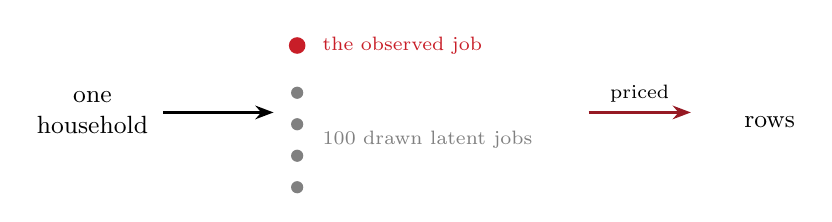
\begin{tikzpicture}[>=Stealth]
  \node[font=\small,align=center] (hh) at (0,0) {one\\household};
  \fill[agenti] (2.6,0.85) circle (3pt);
  \node[agenti,right,font=\scriptsize] at (2.8,0.85) {the observed job};
  \foreach \y in {0.25,-0.15,-0.55,-0.95}{\fill[gray] (2.6,\y) circle (2.2pt);}
  \node[gray,right,font=\scriptsize] at (2.8,-0.35) {\NDrawnJobs{} drawn latent jobs};
  \draw[->,thick] (0.9,0) -- (2.3,0);
  \draw[->,thick,deepred] (6.3,0) -- (7.6,0)
    node[midway,above,font=\scriptsize,black] {priced};
  \node[font=\small,align=center] at (8.6,0) {\NAlternatives\\rows};
\end{tikzpicture}
\end{center}
\vfill
\begin{center}\small
EU-SILC / SRCV 2016 \,\textperiodcentered\, \NHouseholds{} households
\,\textperiodcentered\, \NAlternatives{} alternatives each
\,\textperiodcentered\, \NPricedRows{} priced rows\\[0.6em]
conditional logit with the sampling-of-alternatives correction
\mergedonly{\\[0.7em]
\headline{Every row is priced through the tax--benefit system.}\\[0.3em]
{\small Consumption is computed, not surveyed; the mapping is deterministic.}}
\end{center}
\vfill
\note{[2.0 min] One slide, and deliberately no implementation detail --- no check
counts, no convergence protocol, no hash. \par\medskip
The job space is continuous in wage and hours, so the choice set is sampled rather
than enumerated, and the sampling-of-alternatives correction is what makes the
sampled-set likelihood consistent for the full-set parameters. \par\medskip
Say the one consequence the audience will otherwise trip on: because the observed
row is inserted deterministically and the drawn rows carry a proposal correction,
\textbf{within-set rank and top-k statistics are structurally degenerate here} ---
they are not reported, and their absence is a property of the estimator, not a
weakness being hidden. \par\medskip
If asked about the technical layer, point to the appendix and move on. \par\medskip
25-MIN: MERGE with slide 7 (2.5 combined).}
\end{frame}}

% ==================================================================== 7
% 25-MIN: MERGED into slide 6.  This frame drops in the short deck and
% slide 6 grows the pricing line instead.
\mergedaway{%
\begin{frame}
\frametitle{Pricing: what a job is worth}
\vfill
\begin{center}
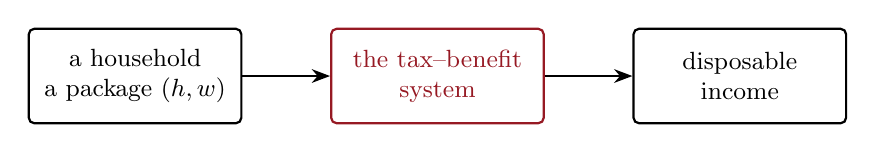
\begin{tikzpicture}[scale=0.96,>=Stealth,
  box/.style={draw,thick,rounded corners=2pt,minimum width=2.7cm,
              minimum height=1.2cm,align=center,font=\small}]
  \node[box] (p) at (0,0) {a household\\a package $(h,w)$};
  \node[box,draw=deepred,text=deepred] (e) at (4.0,0) {the tax--benefit\\system};
  \node[box] (c) at (8.0,0) {disposable\\income};
  \draw[->,thick] (p) -- (e);
  \draw[->,thick] (e) -- (c);
\end{tikzpicture}
\end{center}
\vfill
\begin{center}
\headline{Consumption is computed, not surveyed.}\\[0.5em]
{\small The mapping is deterministic: the same household, hours and wage\\
always return the same euro figure.}\\[0.6em]
\caveat{Nothing in the estimation simulates a tax--benefit outcome.}
\end{center}
\vfill
\note{[2.0 min] This is the slide that makes the counterfactual legitimate, and it
is worth two clean minutes. \par\medskip
EUROMOD is arithmetic: the same household, hours and wage always return the same
euro figure. \textbf{Nothing in the estimation simulates a tax--benefit outcome.}
All the randomness in the pipeline is in \emph{which} points get evaluated, never
in what a point is worth. That is what lets the model price a job the person did
not take. \par\medskip
Mention take-up once --- the minimum-income benefit is granted in full inside the
engine and take-up is applied afterwards as a household trait --- and say why:
take-up is a property of the household, not of the batch it was priced in. \par\medskip
25-MIN: MERGE into slide 6.}
\end{frame}}

% ==================================================================== 8
\shortdeck{%
\begin{frame}
\frametitle{Identification: what is pinned, what stays conditional}
\vfill
\decktable{\small
\renewcommand{\arraystretch}{1.7}
\begin{tabular}{c|c}
\textbf{what the data pin} & \textbf{what stays conditional}\\ \hline
the four availability factors & access \emph{versus} capability\\
the preference block & persistent household heterogeneity\\
the statutory-week peak & \\
\end{tabular}}
\vfill
\begin{center}
\caveat{The decomposition is structural and model-conditional. It is not causal.}
\end{center}
\vfill
\note{[2.0 min] Two conditional items, said plainly. \par\medskip
First, \textbf{the access margin does not separate what a person is capable of from
what the market offers them} --- the estimated access density may combine both, and
this paper claims no ordering between the job-access and earning-opportunity
channels in either direction, even though the point estimates order them and are
printed. \par\medskip
Second, the model carries no persistent household-level term, and slide 9 is why. \par\medskip
Say the general disclaimer once, here: the decomposition is \textbf{structural and
model-conditional, and it is not causal.} \par\medskip
25-MIN: KEEP (2.0) --- and add one sentence of slide 9's lesson: \emph{``three
heterogeneity extensions were tested and all three failed recoverability, for three
different reasons; the backup slide has the design rule.''}}
\end{frame}}

% ==================================================================== 9
\longdeck{%
\begin{frame}
\frametitle{Three heterogeneity extensions}
\vfill
\decktable{\small
\renewcommand{\arraystretch}{1.7}
\begin{tabular}{l|l}
\textbf{extension} & \textbf{what defeats recovery}\\ \hline
random leisure intercept    & no leverage\\
working-alternative frailty & leverage, but no second contrast\\
wage-residual dependence    & no leverage\\
\end{tabular}}
\vfill
\begin{center}
\headline{Depth on an axis is not evidence; only depth on a profile is.}\\[0.4em]
{\small axis 13.56 \quad$\longrightarrow$\quad profile 0.6996 \quad against 2.706}
\end{center}
\vfill
\note{[2.0 min] This is the slide that turns an appendix of failures into a result,
and in a methods-literate audience it is often the most interesting five minutes of
the talk. \par\medskip
All three were specified in advance and assessed by synthetic-recovery diagnostics
\emph{before} any real-data estimation. \par\medskip
Two conditions must hold together for a persistent household-level term to be
identified here. \textbf{Leverage:} the variable it loads on must have enough
within-household spread across the choice set, measured against a scale-one Gumbel,
to reorder a household's own alternatives. The Box--Cox leisure transform has a
within-set spread of 0.073 for men and 0.127 for women --- that is the wall the
random intercept and the wage-residual extension both hit. \par\medskip
\textbf{A second contrast:} even with leverage, the term must move something the
existing coordinates cannot absorb. The frailty term has four times the leverage
and still fails, because a term that shifts every working alternative equally is a
shift the employment intercept can simply re-fit, and with one choice per household
there is no second margin to pin them apart. \par\medskip
Then the punchline: \textbf{depth on an axis is not evidence; only depth on a
profile is.} Holding the rest of the model fixed gives that extension a
likelihood-ratio depth of up to 13.56; re-optimising the rest gives 0.6996, against
the 2.706 a boundary test needs. \par\medskip
Close by saying what this does \emph{not} say: it rejects three parameterisations
on this design, not the existence of heterogeneity. \par\medskip
25-MIN: CUT to backup; fold one sentence into slide 8.}
\end{frame}}

% =================================================================== 10
\shortdeck{%
\begin{frame}
\frametitle{Hours, and the statutory week}
\deckfigtwo{fig01_observed_hours_35h_peak}{observed hours}%
           {fig02_hours_bands_obs_vs_pred}{observed against model-implied}
\begin{center}\small
statutory band \HoursStatObsPct\% observed \,\textperiodcentered\,
\HoursStatPredPct\% model-implied \,\textperiodcentered\,
mean absolute error \HoursMAE{} over \HoursNBins{} bins
\mergedonly{\\[0.35em]
employment \EmpObs{} / \EmpPred{} \,\textperiodcentered\, occupation largest
deviation \OccMaxDev{} \,\textperiodcentered\, bottom offered-wage quintile
over-predicted by 5.3 points}
\end{center}
\note{[2.0 min] Observed \HoursStatObsPct{} per cent in the statutory band against
\HoursStatPredPct{} model-implied; mean absolute error \HoursMAE{} across
\HoursNBins{} bins. \par\medskip
The statutory-week coordinate is the single largest one-coordinate improvement in
the specification --- a likelihood-ratio statistic of 861 on one degree of
freedom. \par\medskip
Then the wording discipline, and use exactly this wording: it is an
\textbf{institutionally motivated opportunity peak in the estimated offer density}.
It is \emph{not} an estimate of the causal effect of the 35-hour statute, and no
counterfactual removing the statute is computed anywhere. \par\medskip
Concede the identified weak spot without being asked: the model under-predicts the
40.5--44.5 band by \HoursBandShortfall{} --- 3.4 points. \par\medskip
25-MIN: MERGE with slide 11 (2.0 combined).}
\end{frame}}

% =================================================================== 11
% 25-MIN: MERGED into slide 10.  This frame drops in the short deck and
% slide 10 grows the employment/occupation/wage line instead.
\mergedaway{%
\begin{frame}
\frametitle{Employment, occupation, and wages}
\deckfigtwo{fig03_employment_obs_vs_pred}{employment}%
           {fig04_occupation_obs_vs_pred}{occupation shares}
\begin{center}\small
employment \EmpObs{} / \EmpPred{} \,\textperiodcentered\,
occupation largest deviation \OccMaxDev{} \,\textperiodcentered\,
median wage fit \WageMedFitMen{} men, $+$\WageMedFitWomen{} women (\euro/h)
\end{center}
\note{[1.5 min] Employment \EmpObs{} observed against \EmpPred{} model-implied.
Occupation: largest deviation across the \OccNCategories{} categories, including
non-employment, is \OccMaxDev{} --- seven-tenths of a percentage point. \par\medskip
Then be straightforward about the wage side, because a referee will find it
anyway: the model \textbf{over-predicts the bottom offered-wage quintile by 5.3
points} and under-predicts the second, third and fourth. \par\medskip
On selected wages the median fit is \textbf{\WageMedFitMen{} euros an hour for men
and $+$\WageMedFitWomen{} for women} --- the model slightly compresses the sex gap
while matching the pooled median to under thirty cents (\WageMedFitAll). \par\medskip
Say that a repair specified in advance was tried --- an hours-conditioned wage
location --- and that it \textbf{failed}: it did not fix the misfit and was not
promoted. \par\medskip
Occupation fit is shown \emph{internally} here for a reason slide 13 explains. \par\medskip
25-MIN: MERGE into slide 10; keep employment, occupation and the wage misfit; drop
the by-sex wage detail.}
\end{frame}}

% =================================================================== 12
\longdeck{%
\begin{frame}
\frametitle{Does the answer depend on the number of drawn jobs?}
\deckfigtwo{figS6_05_key_coefficients_vs_R}{key coordinates, in SE units}%
           {figW05_welfare_vs_R}{the headline contributions}
\begin{center}
\headline{No. Stable from 50 to 400 drawn alternatives.}
\end{center}
\note{[1.0 min] Thirty seconds of content and a minute of credibility. \par\medskip
Every sign is constant and the nested order holds at every rung. \par\medskip
State the one exception rather than claiming uniformity: in the male-reference arm
the preference contribution moves by 1.44 times its own band across the ladder ---
and it is also the object with the tightest band in the study, so the exceedance is
as much about the band as the movement. \par\medskip
The consequence is a reporting rule: \textbf{the male-reference preference
contribution is not quoted to more than two significant figures.} \par\medskip
25-MIN: CUT to backup.}
\end{frame}}

% =================================================================== 13
\shortdeck{%
\begin{frame}
\frametitle{External validation}
\deckfig{figX1_external_hours_lfs_validation}{0.98}
\begin{center}\small
statutory band \ExtStatBandLFS\% external \,\textperiodcentered\,
\ExtStatBandObs\% observed \,\textperiodcentered\,
\ExtStatBandPred\% model-implied
\end{center}
\note{[2.5 min] Frame it before showing it: \textbf{validation only --- no moment
from any external source enters the likelihood, and none of this identifies
anything.} \par\medskip
Panel (b) is the one validation panel: the statutory band takes \ExtStatBandLFS{}
per cent of workers in the external source, \ExtStatBandObs{} in the observed
sample and \ExtStatBandPred{} model-implied, and the concentration is larger for
women than men in all three (\ExtStatBandLFSWomen{} against
\ExtStatBandLFSMen{} externally) --- which the model reproduces \textbf{without any
sex-specific hours coordinate}. \par\medskip
Then draw the line the evidence supports and no further: \textbf{the validation
claim is limited to the hours-distribution feature for which the model and the
external source have commensurable objects --- in particular the statutory-band
concentration.} \par\medskip
The EU-LFS wish-more-hours and desired-minus-actual-hours profiles, panels (a) and
(c), are \textbf{separate descriptive context}. Because the model has no
desired-hours or underemployment counterpart, they are not interpreted as model
predictions or as validation of the estimated opportunity weights, and no
association between them and any estimated quantity is computed or shown. Report
them descriptively if asked --- \WishLFS{} per cent of employed people in the
priced bands report wanting more hours, declining with hours worked
(\ExtWishStatBand{} per cent at the statutory band, \ExtWishLongHours{} at long hours) --- and
stop there. \par\medskip
Two things not to skip. The external population is all adults aged 20--60 while the
sample is single-adult households, so \textbf{a gap here is a population
difference, not a prediction error}. And the matched employer--employee earnings
source is simply not available in the accessible data, so no external wage
comparison is attempted and none is faked. \par\medskip
25-MIN: compress to 1.0 --- panel (b) and the population caveat; drop panel (a).}
\end{frame}}

% =================================================================== 14
\shortdeck{%
\begin{frame}
\frametitle{The welfare measure, and two real households}
\deckfig{figE1_matched_pair}{0.94}
\begin{center}\small
same preference profile (\EOneOmegaA{} and \EOneOmegaB) \,\textperiodcentered\,
employment probability \textcolor{agenti}{\EOnePiA} against
\textcolor{agenth}{\EOnePiB}
\end{center}
\note{[1.5 min] Define the measure in one sentence and say what normative choice it
encodes: what flat consumption level, available at every job in this household's
\textbf{ex-ante estimated opportunity distribution}, would leave them as well off
as they are --- so pay is compensated and the set is the household's own
responsibility. \par\medskip
Say ``estimated opportunity distribution'', not ``the household's own set'': the
empirical object is a density the model estimates, not an observed menu, and the
welfare integral is taken over it ex ante rather than over realised draws. \par\medskip
Then the pair, and stress that it was \textbf{selected by a rule fixed before any
household was looked at}, from \EOneNPairs{} admissible pairs matched on observed
employment, occupation, hours band and wage quintile: two single men, both working
\EOneHours{} hours in the same occupation in the same wage quintile, whom the model
gives essentially the same preference profile --- leisure weights \EOneOmegaA{} and
\EOneOmegaB{} --- and very different opportunity: \textbf{employment probability
\EOnePiA{} against \EOnePiB}. \par\medskip
Point at where the difference is \emph{not}: their median wage offers are
\euro11.38 and \euro11.05, within thirty cents. The whole gap is on the
participation margin, which is where region, urbanisation and the local
unemployment rate enter --- so this pair is the household-level face of the
geographic split on slide 17. \par\medskip
This is slide 3's panel (a) on real estimates. Repeat once that these panels are
\textbf{densities, not job draws}. \par\medskip
If asked how this pair was chosen, or why it differs from an earlier version: a
defect in the selection code left the ranking's opportunity distance without the
region term. It is repaired, the ranking was re-run over the same admissible pairs
under the same rule, and this is what it returns --- a cleaner pair, separated by
\EOneSeparation$\times$ rather than 2.08$\times$, whose gap is geographic rather
than in the wage offer. \textbf{No number in the welfare decomposition moved}; the
defect was confined to this illustration. \par\medskip
25-MIN: KEEP (1.5) --- the measure and the pair, no panel walk-through.}
\end{frame}}

% =================================================================== 15
\shortdeck{%
\begin{frame}
\frametitle{The headline}
\only<1>{\deckfig{figW02_headline_decomposition}{0.92}}
\only<2>{\deckfig{figU01_headline_two_intervals}{0.92}}
\begin{center}
\onslide<1->{\headline{\Env{} \wband{\ShareEnv}{\BandEnv}\%
\quad\textperiodcentered\quad \Pref{} \wband{\SharePref}{\BandPref}\%}}\\[0.3em]
\onslide<2->{\caveat{parameter interval: \pref{} [\ParPrefLo, \ParPrefHi] \quad
\env{} [\ParEnvLo, \ParEnvHi]}}
\end{center}
\note{[2.5 min] Read the sentence as it is written, because it is generated from
the table with a guard and its qualifiers are not decoration: \emph{within the
currently modelled non-preference environment, budget-side endowments and needs are
the largest nested contribution under both positive models and both
reference-preference conventions.} \par\medskip
Baseline inequality is a Gini of \IBaselineShort; equalising the environment alone
takes it to \IEnvOnlyShort{} (equalising preferences alone \emph{raises} it, to
\IPrefOnly); equalising both takes it to numerical zero --- and that
last point is a \textbf{tested property, not an assumption}: the fully common state
is zero to machine precision, which is what licenses reporting shares at all. \par\medskip
Then the licensed reading, which must be said out loud: \textbf{no channel
``explains'' a percentage.} A contribution is the value of an equalisation operator
in a cooperative game --- the form is \emph{equalising this channel removes this
share of baseline inequality} --- not a variance share and not a causal effect. \par\medskip
CLICK 2. Be exact about the bars, because there are now \textbf{two kinds} and they
must not be read as one. The \textbf{integration band} says how well the nodes
integrate the model at a fixed parameter vector. The \textbf{parameter interval}
says how much the estimate would move across samples --- propagated from the
cluster-robust asymptotic distribution, \textbf{not a bootstrap}, nothing resampled
and nothing re-estimated. They are drawn on offset rows and are \textbf{never
merged}; the shaded union is not a confidence interval. \par\medskip
The parameter interval is the wider by \ParWidenLo{} to \ParWidenHi{} times, so the
preference share is \SharePref{} per cent with an interval of
\textbf{[\ParPrefLo, \ParPrefHi]} and the environment share \ShareEnv{} with
\textbf{[\ParEnvLo, \ParEnvHi]} --- the environment stays dominant across it, and
the sign of the preference contribution does not change within it. Every parameter
interval is \textbf{conditional on the active set} at the estimated parameter
vector, over \ParKInterior{} draws from the asymptotic sampling
distribution. \par\medskip
One counter-intuitive fact worth 30 seconds if the room is engaged: equalising
preferences \emph{raises} measured inequality, because the households with the
worst opportunity sets are the ones whose own tastes currently do most to reconcile
them to those sets. \par\medskip
25-MIN: KEEP (2.5) --- this is the slide the talk exists for.}
\end{frame}}

% =================================================================== 16
\shortdeck{%
\begin{frame}
\frametitle{Inside the environment}
\deckfig{figW03_nested_environment}{0.92}
\begin{center}\small
\Needs{} \wband{\ShareNeeds}{\BandNeeds}\% \,\textperiodcentered\,
\Earn{} \wband{\ShareEarn}{\BandEarn}\% \,\textperiodcentered\,
\Acc{} \wband{\ShareAcc}{\BandAcc}\%\\[0.4em]
\headline{market side together: \wband{\ShareMarket}{\BandMarket}\%}
\end{center}
\note{[1.5 min] Endowments and needs \ShareNeeds{} per cent (plus or minus
\BandNeeds), earning opportunities \ShareEarn{} (\BandEarn), job access
\ShareAcc{} (\BandAcc) --- so the two market-side channels together are
\textbf{\ShareMarket{} per cent (\BandMarket)}, and that combined figure is
reported separately from endowments and needs on purpose. \par\medskip
Two disciplines. First, \textbf{do not say job opportunities explain the
environment share}: the environment is the \emph{complete} non-preference
environment, and the market-side part of it is a third, not all of it. \par\medskip
Second, \textbf{no ordering is claimed between job access and earning
opportunities} --- the point estimates order them and are printed, but the access
margin is exactly the one that does not separate capability from availability, so
an ordering claim would be a claim about something the design does not
identify. \par\medskip
If asked why the budget channel is so large, give the honest reading: this is
France 2016, a system with substantial means-tested transfers, and the result is
partly a statement about that system. It is not portable without
re-estimation. \par\medskip
25-MIN: KEEP (1.5) --- the three numbers, the combined market-side figure, and the
no-ordering rule.}
\end{frame}}

% =================================================================== 17
\longdeck{%
\begin{frame}
\frametitle{Inside job access: it is almost all geography}
% two caption lines here, so the figure box is one step shorter than
% \deckfig's default to keep the frame from overflowing
\only<1>{\begin{center}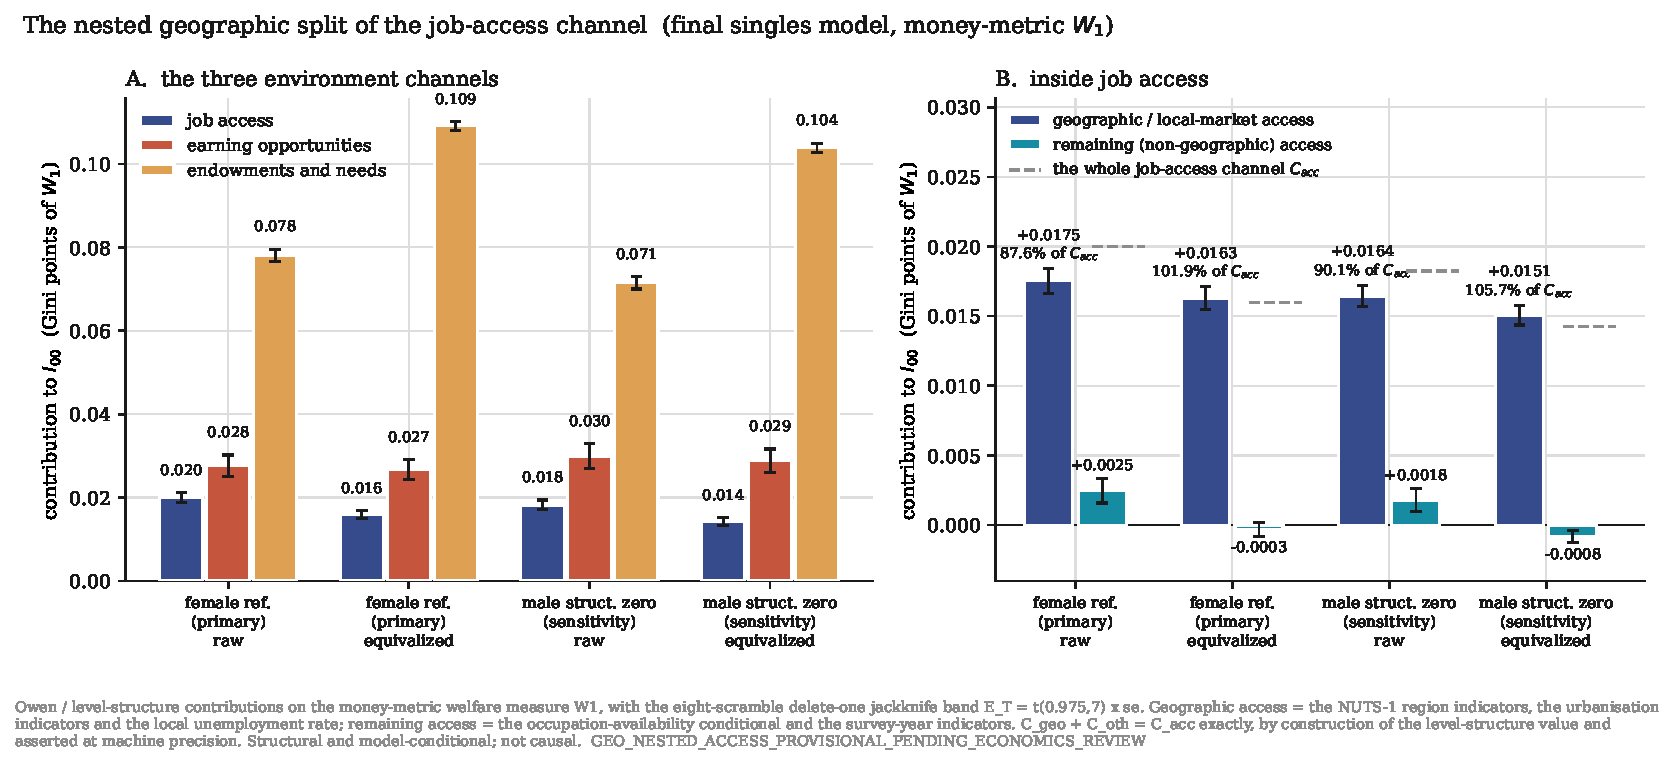
\includegraphics[width=0.90\textwidth,height=0.64\textheight,%
  keepaspectratio]{figG01_nested_geographic_access}\end{center}}
\only<2>{\begin{center}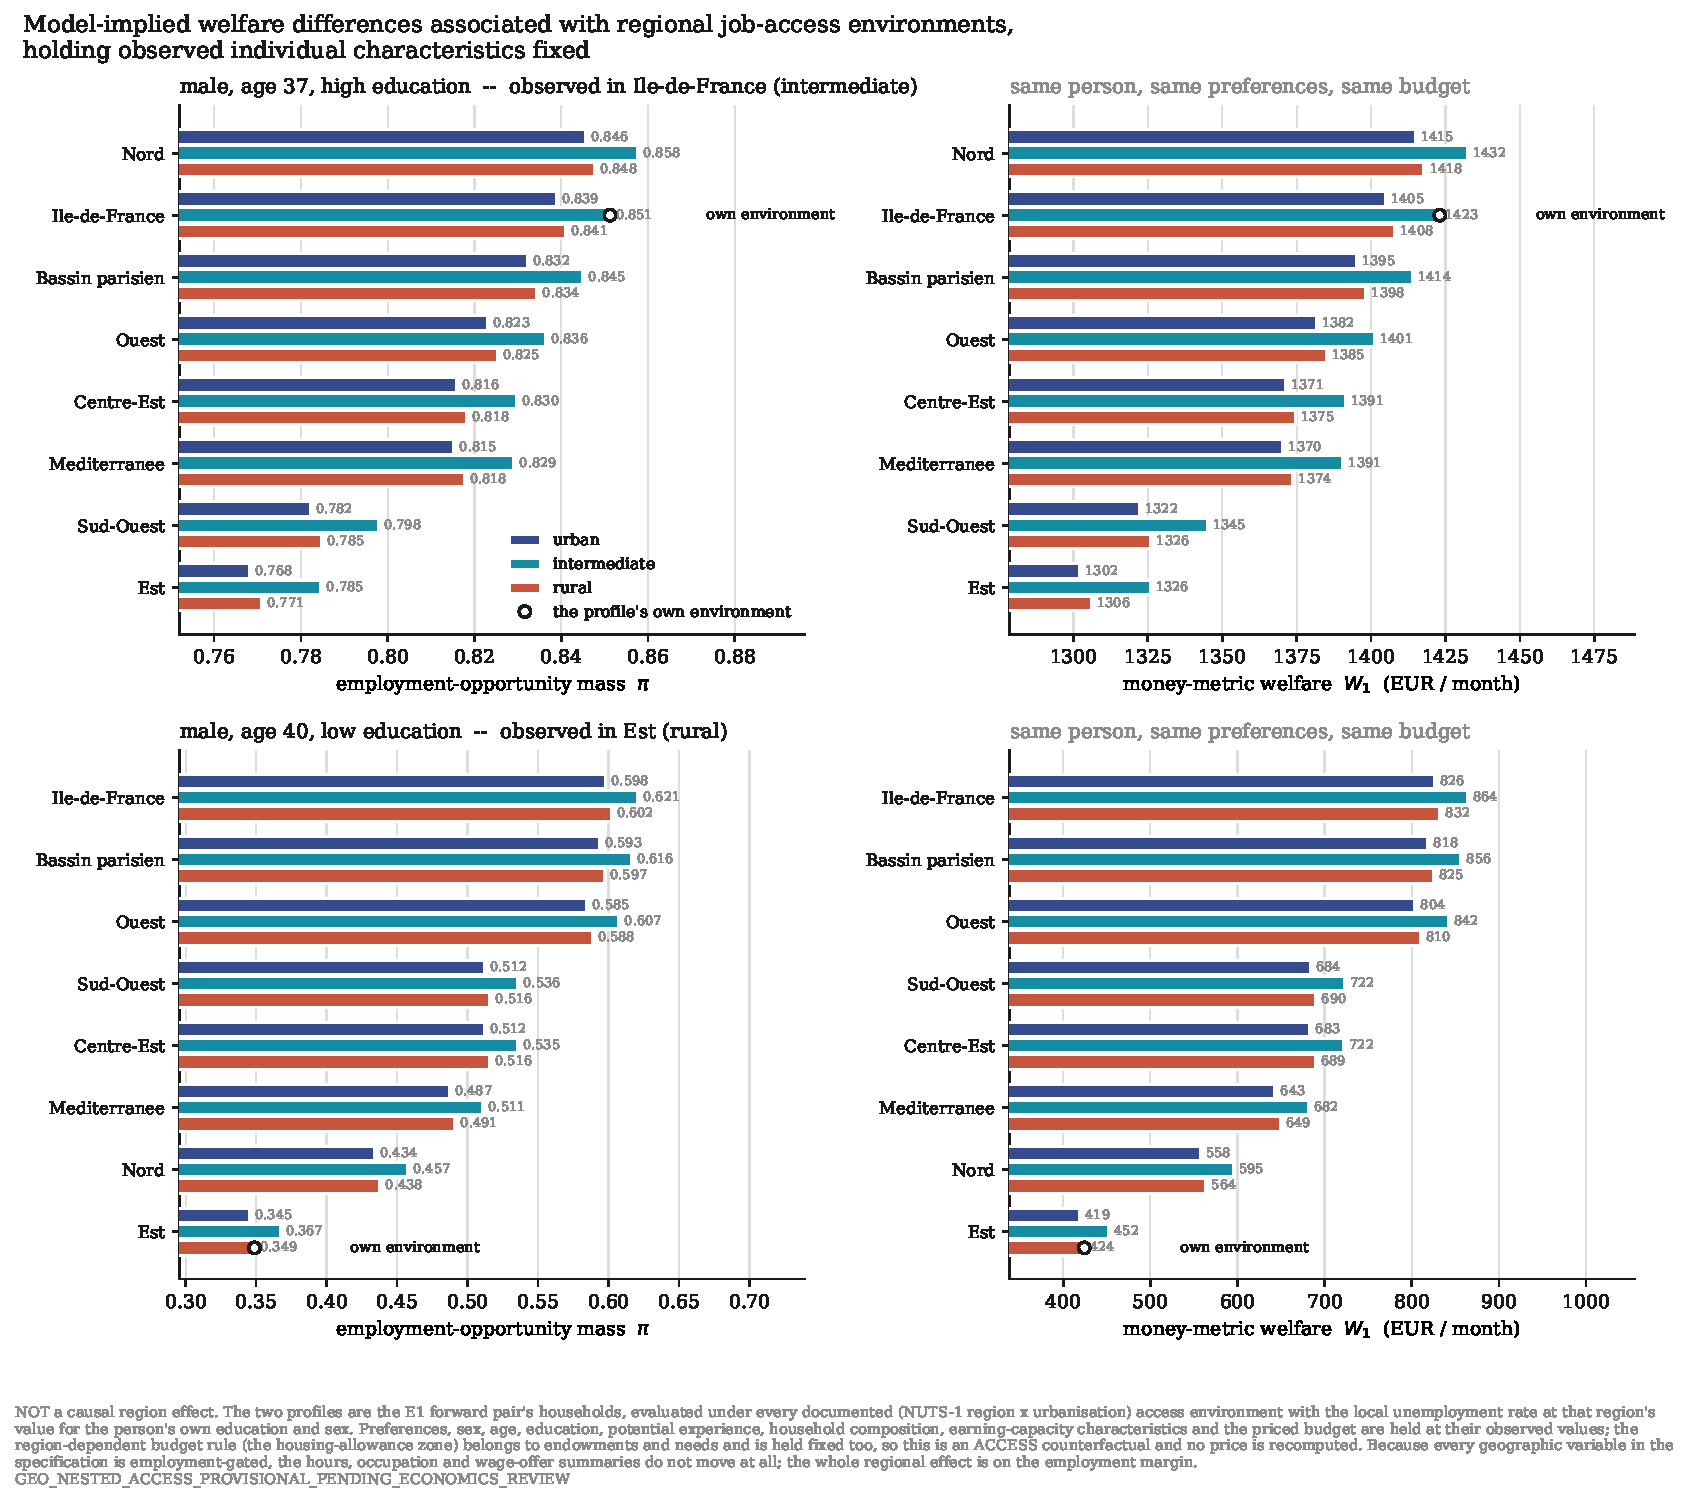
\includegraphics[width=0.90\textwidth,height=0.64\textheight,%
  keepaspectratio]{figG02_regional_access_environments}\end{center}}
\begin{center}\footnotesize
geographic access \wband{\ShareGeoRaw}{\BandGeoRaw}\% raw,
\wband{\ShareGeoEqv}{\BandGeoEqv}\% equivalized \,---\,
\GeoShareOfAccRaw\% and \GeoShareOfAccEqv\% of \acc\ \ \caveat{[\ParGeoShareLo,
\ParGeoShareHi]}\\
\caveat{This is not a finding that region drives welfare inequality.}
\end{center}
\note{[2.0 min] Two numbers and one caveat, and the caveat is the point. \par\medskip
Equalising the geographic access environment removes \textbf{\ShareGeoRaw{} per
cent (\BandGeoRaw)} of baseline inequality on the raw basis and \ShareGeoEqv{}
(\BandGeoEqv) equivalized, against a whole job-access channel of
\ShareAccNestedRaw{} and \ShareAccNestedEqv. So geography is
\textbf{\GeoShareOfAccRaw{} per cent (\BandGeoShareOfAccRaw)} of the channel raw
and \GeoShareOfAccEqv{} (\BandGeoShareOfAccEqv) equivalized. \par\medskip
\textbf{Never say that ratio without its parameter interval ---
[\ParGeoShareLo, \ParGeoShareHi] per cent on the raw basis.} It is a ratio of two
contributions one of which is small, so its sampling distribution is much wider
than its integration band suggests. \par\medskip
Say why a share can exceed one before anyone asks: shares here are \textbf{signed
and never renormalised}, so the residual is negative on the equivalized rows, not
missing. \par\medskip
Then the caveat, delivered as a limitation of the specification rather than as a
result. The two sub-players do not have comparable support. The geographic block
varies household by household over eight regions, three urbanisation categories and
a region-education-sex unemployment rate. The remaining access block is the
occupation-availability conditional, and this specification conditions it on
\textbf{sex alone} --- a two-cell table --- plus year indicators that are
identically zero on a one-year sample. Almost all the between-household dispersion
the access operator \emph{can} remove is geographic \textbf{by construction}. The
honest reading is about the composition of the access block, not about the
importance of place. \par\medskip
And the sentence that stops the obvious misreading: \textbf{this is not a finding
that region drives welfare inequality.} Job access as a whole is \ShareAcc{} per
cent of measured inequality raw and \ShareAccEqv{} equivalized, against
\ShareNeeds{} and \ShareNeedsEqv{} for endowments and needs. If asked about
regional policy: the only regional dependence in the tax-benefit system here is the
housing-allowance zone, and that belongs to endowments and needs, deliberately
outside this split. \par\medskip
CLICK 2 --- optional, and the first thing to drop. This takes the two matched
households of slide 14 and moves them across all \NRegionalEnvs{} region $\times$
urbanisation environments, holding preferences, demographics, earning-capacity
characteristics, the priced budget and the region-dependent budget rule fixed --- an
access counterfactual with no price recomputed. The high-education man's
employment-opportunity mass runs \RegMassALo{} to \RegMassAHi{} and his welfare
\euro\RegWelfALo{} to \euro\RegWelfAHi; the low-education man's,
\textbf{\RegMassBLo{} to \RegMassBHi} and \textbf{\euro\RegWelfBLo{} to
\euro\RegWelfBHi}. Handle that second range carefully if you show it: it is not
that moving would double his welfare, it is that a household already at a low
participation probability sits on the steep part of the map from access index to
employment margin, and his own environment is the least favourable of the
twenty-four. \par\medskip
Because every geographic variable here enters only when the household works, the
whole regional difference is \textbf{on the employment margin}. Say the label out
loud --- \textbf{this is not a causal region effect}; nothing here identifies what
would happen to someone who moved. \par\medskip
25-MIN: CUT to backup.}
\end{frame}}

% =================================================================== 18
\longdeck{%
\begin{frame}
\frametitle{Job access does more of the work among men}
\deckfig{figU02_subgroup_decomposition}{0.92}
\begin{center}\small
\acc{}: \wband{\SubAccMen}{\SubAccBandMen}\% of men's measured inequality against
\wband{\SubAccWomen}{\SubAccBandWomen}\% of women's\\[0.3em]
\caveat{Men's \pref{} share: \SubPrefMenFemRef\% and \SubPrefMenMaleRef\%
across the two reference conventions --- a sign change. No sign statement is
licensed.}
\end{center}
\note{[1.5 min] Say what the estimand is before the number, because it is easy to
hear as something else. Every reference object is computed \textbf{once over the
whole population and is common to every group}, so a bar answers \emph{how much of
this group's own inequality is removed by moving its households to the common
population reference}. It is a \textbf{within-subgroup} decomposition, not a
contribution of the characteristic: nothing here splits inequality into
between-sex and within-sex parts, and nothing here is causal. \par\medskip
The finding: \textbf{job access carries \SubAccMen{} per cent of men's measured
inequality against \SubAccWomen{} of women's} --- and it holds under both reference
conventions and on both bases, \SubAccMenMaleRef{} against \SubAccWomenMaleRef{}
under the male reference, \SubAccMenEqv{} against \SubAccWomenEqv{}
equivalized. The geographic part is larger for men too, \SubGeoMen{} against
\SubGeoWomen. \par\medskip
Say carefully what it does not mean: it is not that men face worse access, because
the decomposition is not a level comparison. It is that the dispersion of access
within men does more of the work among men than the dispersion of access within
women does among women. \par\medskip
\textbf{Then the disclosure, and do not skip it.} The men's preference share is
\SubPrefMenFemRef{} per cent under the female reference and \SubPrefMenMaleRef{}
under the male one. That is a \textbf{sign change}, not a magnitude sensitivity,
and \textbf{no statement about the sign of the male preference contribution is
licensed} --- so make none. It is worth pausing on: the population preference share
is positive under both conventions, so the headline's sign stability does not
extend to every subgroup of it. This is the sharpest demonstration in the talk of
how much rides on a normative choice. \par\medskip
If asked about other splits: urbanisation and children were computed on the same
construction, neither carries a finding that survives the same scrutiny, and both
are in the appendix. \par\medskip
25-MIN: CUT to backup.}
\end{frame}}

% =================================================================== 19
\shortdeck{%
\begin{frame}
\frametitle{What a conventional model would have found}
\deckfig{figR01_benchmark_decomposition}{0.92}
\begin{center}\small
\pref{} share \BenchSharePrefRUMB\% against \BenchSharePrefRURO\%
\,\textperiodcentered\, measured inequality \BenchInequalityDropRaw\% raw
\,\textperiodcentered\, sex leisure gap $+0.428 \to -1.991$
\end{center}
\note{[2.5 min] This is the paper's own counterfactual about method and it is worth
doing properly, because \textbf{the result is not the one the premise predicts} and
saying so is what makes the rest credible. \par\medskip
Set it up in one line: every household-indexed argument of the availability object
is replaced by a common value, so the benchmark is a conventional model with hours
constants, a fixed cost of work and a sex-specific leisure block --- what a careful
analyst without an opportunity object would have fitted. \par\medskip
Then three findings, in this order. \textbf{First, fit does not separate them.} The
benchmark is \BenchGapNats{} nats worse on the objective (\BenchNegLL{} against
\PrefNegLL{} over \PrefNFree{} free parameters; a likelihood-ratio statistic of
\BenchLR{} on \BenchDF{} degrees of freedom, quoted as an upper bound because the
benchmark is not nested), but its marginal fit is \emph{as good or better} --- hours 0.0080
against 0.0083, occupation 0.0029 against 0.0034, wage quintiles 0.0203 against
0.0261. A referee judging on marginal fit alone would prefer the model with no
opportunity object in it. That is the argument for not judging on marginal fit
alone. \par\medskip
\textbf{Second, the availability information goes into the taste parameters.} The
\BenchNConstants{} hours-band constants reappear in the benchmark's \emph{utility}
index at essentially their availability values --- mean absolute difference
\BenchConstMAD. The same constants, read twice. And the male-minus-female leisure
gap \textbf{reverses sign}, from $+0.428$ to $-1.991$: measured leisure preference
shifts toward the group facing the worse offer environment, exactly as the confound
predicts. \par\medskip
\textbf{Third --- and this is the honest surprise --- the preference share of the
welfare decomposition barely moves}: \BenchSharePrefRUMB{} per cent under the
benchmark against \BenchSharePrefRURO{} under the preferred model. The omitted
market-side share does not become taste. It mostly leaves the total --- measured
inequality falls \BenchInequalityDropRaw{} per cent on the raw basis and
\BenchInequalityDropEqv{} equivalized --- and what stays is relabelled onto
endowments and needs. \par\medskip
Say the licensed sentence: \emph{behavioural coefficients can absorb omitted
availability structure; omitting heterogeneous opportunities materially lowers
measured money-metric inequality; the welfare-decomposition preference share
changes little; and the missing opportunity contribution is reallocated primarily
within the non-preference environment rather than into preferences.} \par\medskip
Do \textbf{not} claim it demonstrates a large welfare-level preference-misattribution
effect. \par\medskip
If asked why that matters for the paper's contribution: the case for an opportunity
object is not that it rescues the decomposition from attributing everything to
taste --- on this measure it does not. It is that without one the estimated
preferences point the wrong way, the level of inequality is understated by a fifth
to a quarter, and the environment's composition is misdescribed. \par\medskip
25-MIN: compress to 1.5 --- the reversed sex gap and the preference-share result;
drop the fit comparison.}
\end{frame}}

% =================================================================== 20
\shortdeck{%
\begin{frame}
\frametitle{What is fragile, and what is not}
\vfill
\decktable{\small
\renewcommand{\arraystretch}{1.7}
\begin{tabular}{l|c|c}
\textbf{perturbation} & \textbf{\pref{} share} & \textbf{\env{} side}\\ \hline
reference-preference convention & \SharePref{} $\to$ \SharePrefMaleRef\% & $<3.5\%$\\
a bound on a preference curvature & $\approx 13\%$ move & $<3.5\%$\\
pinning the couples male leisure block & up to $73\%$ move & $<3.5\%$\\
\end{tabular}}
\vfill
\begin{center}
\caveat{No sign and no ordering changes anywhere. Market-side total
\ShareMarket\% against \ShareMarketMaleRef\% across references.}
\end{center}
\vfill
\note{[2.0 min] This is the most useful slide for a critical audience and it is a
strength, not a concession. \par\medskip
\textbf{Be precise about which perturbation produces which range --- they are
different objects and it is easy to conflate them.} \par\medskip
Changing only the reference-preference convention on the preferred singles model
moves the preference contribution from \textbf{\SharePref{} to \SharePrefMaleRef{}
per cent on the raw basis} and from \textbf{\SharePrefEqv{} to
\SharePrefEqvMaleRef{} per cent on the coalition-consistent equivalized basis}.
These paired values are reported as ranges and never averaged. \par\medskip
The broader \textbf{\SharePrefEnvLo--\SharePrefEnvHi{} per cent} envelope is across
all eight rows of the exact table and therefore also reflects the positive-model
and equivalization choices; \textbf{it is not a reference-only range}. \par\medskip
The other two perturbations: the age-bound diagnostic moves the preference share by
about 13 per cent, and pinning the couples male leisure block moves it by up to 73
per cent. The environment side moves by under 3.5 per cent in all of them, and no
sign and no ordering changes anywhere. \par\medskip
The market-side total is nearly unchanged across reference conventions ---
\ShareMarket{} against \ShareMarketMaleRef{} per cent on the raw basis --- so
reference sensitivity is concentrated in the preference/environment split rather
than in the environment's internal structure. \par\medskip
25-MIN: KEEP (1.5) --- the three rows and the range rule; absorb two sentences of
slide 22.}
\end{frame}}

% =================================================================== 21
\shortdeck{%
\begin{frame}
\frametitle{Couples}
\deckfigtwo{figC02_couples_decomposition}{the couples decomposition}%
           {figC03_singles_vs_couples}{singles and couples, equivalized}
\begin{center}\small
2,275 couples \,\textperiodcentered\, same nested order, same \env{} dominance\\[0.3em]
\caveat{The couples \pref{} share is not structurally robust. Singles remain the
quantitative headline.}
\end{center}
\note{[2.0 min] 2,275 opposite-sex couples, one specification and no search. \par\medskip
Lead with the finding that was not targeted and is the most striking piece of
internal consistency in the paper: the \textbf{female statutory-week peak in
couples reproduces the singles value to within three hundredths} --- 2.5474 against
2.5795, a third of a standard error --- on a different frame, a different choice set
and a joint likelihood. \par\medskip
Then the substance: same nested order on both bases, same environment
dominance. \par\medskip
Then the discipline, and do not soften it. Synthetic-recovery diagnostics
identified the male leisure block as the weakly recovered part of the couples
specification \emph{before} the welfare sensitivity exercise was run, and that
exercise confirms it bites: the preference contribution moves by up to 73 per cent,
so \textbf{no single couples preference percentage is presented as structurally
robust}, and every couples preference figure travels with its range. \par\medskip
One directional difference from singles, stated because it is real: for couples,
equalising preferences \emph{reduces} measured inequality, the opposite of the
singles result, so the singles interpretation does not transfer. \par\medskip
If asked about pooling: pooled equivalized inequality is well defined and reported,
but the pooled \emph{decomposition} is not exhaustive --- the two household types
have different reference bundles, so the fully common pooled state is 39.4 per cent
of the pooled baseline. That is an \textbf{open welfare-reference question, not a
numerical failure}. \par\medskip
25-MIN: compress to 1.0 --- the statutory-week replication, the same order, and the
sensitivity caveat.}
\end{frame}}

% =================================================================== 22
\longdeck{%
\begin{frame}
\frametitle{Limits, and what would identify more}
\vfill
\decktable{\small
\renewcommand{\arraystretch}{1.7}
\begin{tabular}{l|l}
\textbf{limit} & \textbf{what would change it}\\ \hline
access versus capability & external job-offer or access-rate moments\\
persistent heterogeneity & repeated choices per household\\
no desired-hours target & external desired-hours moments\\
one country, one year, one system & re-estimation; no portability claimed\\
\end{tabular}}
\vfill
\begin{center}
\caveat{Multi-adult households are excluded. Welfare magnitudes are provisional
pending one bounded economics review.}
\end{center}
\vfill
\note{[1.5 min] Four limits, thirty seconds each at most. \par\medskip
\textbf{Access versus capability} --- separating them needs external moments on
job-offer or access rates. \par\medskip
\textbf{Persistent heterogeneity} --- needs repeated choices per household, which
would supply the second contrast slide 9 showed is missing. \par\medskip
\textbf{The hours block has no desired-hours target} --- external desired-hours
moments would discipline it against a stated target rather than inferring both from
realised hours. \par\medskip
\textbf{One country, one year, one system} --- nothing here is portable without
re-estimation, and no portability is claimed. \par\medskip
Say the honest scope line: multi-adult households are excluded, and their admission
needs five assumptions this design leaves unstated. Also state, once, that the
welfare magnitudes are \textbf{provisional pending one bounded economics
review}. \par\medskip
25-MIN: CUT --- fold two sentences into slide 20 and slide 23.}
\end{frame}}

% =================================================================== 23
\shortdeck{%
\begin{frame}
\frametitle{Conclusion}
\vfill
\begin{itemize}\itemsep1.1em
  \item<1-> \textbf{The method.} A household-specific opportunity distribution
        estimated jointly with \pref, every job priced through the real
        tax--benefit system.
  \item<2-> \textbf{The finding.} \Env{} carries \ShareEnv\% of measured
        money-metric welfare inequality; inside it the budget side carries more
        than the market side.
  \item<3-> \textbf{The margin.} The \pref{} share is the fragile quantity:
        \SharePref\% to \SharePrefMaleRef\% across the two normative conventions.
\end{itemize}
\vfill
\note{[1.0 min] Close on the contribution rather than the number. \par\medskip
The method: a household-specific opportunity distribution estimated jointly with
preferences, with every job priced through the real tax--benefit system, and a
decomposition that is exhaustive \textbf{by measurement rather than by assumption}
--- the fully common state is numerically zero. \par\medskip
The finding: the non-preference environment carries roughly nine-tenths of measured
money-metric welfare inequality (\ShareEnv{} per cent), and inside it the budget
side carries more than the market side (\ShareNeeds{} against \ShareMarket). \par\medskip
The margin: the preference share is the fragile quantity, it is reported as a range
across the two normative conventions (\SharePref{} to \SharePrefMaleRef{} per
cent), and it is where the next round of evidence should go. \par\medskip
Then stop talking. \par\medskip
25-MIN: KEEP (1.0) --- absorb the two limits sentences.}
\end{frame}}

% ====================================================================
% BACKUP SLIDES.  Not in the running order; each held for one question.
% \appendix keeps the main frame total at the running-order count.
% ====================================================================
\appendix

% ---------------------------------------------------------------- B1
\begin{frame}
\frametitle{B1 --- The estimated coefficients}
\deckfig{fig08_coefficients_by_block}{0.92}
\begin{center}\small
\NEstimatedParams{} estimated structural parameters, robust 95\% intervals
\end{center}
\note{Held for: \emph{``What are the actual parameter estimates?''} \par\medskip
The final singles model carries \textbf{\NEstimatedParams{} estimated structural
parameters}. The full table with standard errors is in the paper's Appendix A. \par\medskip
Read off the two things worth reading: the leisure curvatures differ sharply by sex
and are precisely estimated, and the occupation-availability weights differ
strongly by sex --- men concentrated in and around routine manual, women's
availability tilted toward nonroutine cognitive. That sex-specific structure is what
keeps occupational sorting out of the taste block. \par\medskip
Note that two coordinates rest on an active bound and carry no standard error, and
that the ten pinned coordinates are not displayed.}
\end{frame}

% ---------------------------------------------------------------- B2
\begin{frame}
\frametitle{B2 --- Exhaustiveness: how the decomposition was made to close}
\vfill
\decktable{\small
\renewcommand{\arraystretch}{1.6}
\begin{tabular}{l|l}
\textbf{defect} & \textbf{what fixed it}\\ \hline
a missing budget channel & added as a fourth player from its own marginals\\
asymmetric money-metric inversion & reference side moves with the coalition\\
an incomplete male reference block & structural zero on the child leisure term\\
\end{tabular}}
\vfill
\begin{center}
\headline{Exhaustiveness here is a tested property, pre-stated before any cell was read.}\\[0.4em]
{\small the fully common state is \IBothCommon{} --- numerically zero}
\end{center}
\vfill
\note{Held for: \emph{``Why should I believe the four channels are exhaustive?''}
--- and it is the best question in the room. \par\medskip
This is a methodological result and it should be told as one, because the honest
answer is that it did \textbf{not} close at first. An earlier implementation failed
the exhaustiveness test on both limbs in every arm --- equalising everything left an
index \textbf{three times} the one it started from --- and the headline was correctly
\textbf{halted}. \par\medskip
Three things were found and removed. A missing budget channel, added as a fourth
player formed from its own marginals rather than as a relabelled residual. An
asymmetry in the money-metric inversion, where the reference side was frozen at the
baseline while the attained side moved with the coalition; correcting it removed
about 95 per cent of the residual. And a male reference block that was incomplete,
because the specification carries a children-in-leisure term for women and none for
men. \par\medskip
With all three fixed the fully common state is numerically zero.
\textbf{Exhaustiveness here is a tested property, and the test was pre-stated
before any cell was read.}}
\end{frame}

% ---------------------------------------------------------------- B3
\begin{frame}
\frametitle{B3 --- Equivalization, and why the scale has to move}
\vfill
\decktable{\small
\renewcommand{\arraystretch}{1.25}
\begin{tabular}{l|c|c}
 & \textbf{raw} & \textbf{equivalized}\\ \hline
\pref & \SharePref\% & \SharePrefEqv\%\\
\env & \ShareEnv\% & \ShareEnvEqv\%\\ \hline
\acc & \ShareAcc\% & \ShareAccEqv\%\\
\earn & \ShareEarn\% & \ShareEarnEqv\%\\
\needs & \ShareNeeds\% & \ShareNeedsEqv\%\\ \hline
market side & \ShareMarket\% & \ShareMarketEqv\%\\
\end{tabular}}
\vfill
\begin{center}
\caveat{Freezing each household's own scale leaves a residual of 0.071799 ---
precisely the weighted Gini of one over the scale.}
\end{center}
\vfill
\note{Held for: \emph{``You divide by an equivalence scale --- doesn't that break
the decomposition?''} \par\medskip
It does, under the natural convention, and exactly: freezing each household's own
scale in all states leaves a residual of 0.071799, which is \textbf{precisely the
weighted Gini of one over the scale} --- the same number to six decimals. Dividing a
common numerator by a household-specific divisor reintroduces exactly the
dispersion of the divisor. \par\medskip
The fix is the one the inversion already legislates: household composition
\textbf{is} an endowments-and-needs object, so the scale moves with the channel that
equalises composition, and exhaustiveness is restored exactly. \par\medskip
Equivalizing raises measured inequality by about a fifth and changes no qualitative
conclusion, but it does move the market-side total from \ShareMarket{} to
\ShareMarketEqv{} per cent --- both are reported and neither is ``the'' answer. \par\medskip
Then the normative point, and state the justification as \textbf{factor
consistency, not closure}: the scale moves because household composition is itself
part of the endowments-and-needs factor being equalised --- the equivalence scale is
a function of that composition and is therefore recomputed at the
coalition-specific needs profile. \textbf{Exact closure is a consequence of this
definition, not its justification.} \par\medskip
If instead the normative object were to equalise resources while leaving needs
fixed, the household's own scale would remain and the residual would be a genuine
needs component requiring different accounting. That alternative is coherent; this
paper adopts the first object.}
\end{frame}

% ---------------------------------------------------------------- B4
\begin{frame}
\frametitle{B4 --- Why the hours-wish evidence is context, not a moment}
\vfill
\decktable{\small
\renewcommand{\arraystretch}{1.7}
\begin{tabular}{l|l}
\textbf{ground} & \textbf{what it shows}\\ \hline
definitional & the candidate's optimum tracks pay: 98.1\% pay more, median 2.58$\times$\\
identification & the hours block moves the moment by \textbf{exactly 0}\\
numerical & \WishModel\% against \WishLFS\%; the profile does not match\\
\end{tabular}}
\vfill
\begin{center}
\caveat{Steelman (own $\pm5\%$ wage neighbourhood): 19.4\% --- and the hours block
is exactly as inert.}
\end{center}
\vfill
\note{Held for: \emph{``You have external data on who wants more hours --- why not
use it to discipline the hours block?''} \par\medskip
The honest answer is that it was tried and there is no counterpart to compare
against. Three independent grounds. \par\medskip
\textbf{Definitional:} the survey asks about more hours \emph{at the current wage},
and the frame has no such menu --- exactly one node per household carries the
observed wage, the chosen one, so the candidate's optimum tracks pay, paying more
for 98.1 per cent of workers at a median 2.58$\times$ the observed wage. \par\medskip
\textbf{Identification, and this is the decisive one:} perturbing any of the six
hours-opportunity coefficients moves the moment by \textbf{exactly zero} and moves
not one household's optimum --- removing the opportunity weights removes the very
block the moment was meant to discipline. \par\medskip
\textbf{Numerical:} the level can be made to agree and the profile cannot;
\WishModel{} per cent against \WishLFS, but the external share falls monotonically
in hours and the model's does not, and the model puts none at long hours against
\ExtWishLongHours{} per cent. \par\medskip
The steelman was tried: restricting to the household's own $\pm5$ per cent wage
neighbourhood fixes the pay artefact and brings the aggregate to 19.4 per cent ---
closer than the model deserves --- and the hours block is \emph{exactly as
inert}. \par\medskip
The fork is architectural: a definition that removes the opportunity weights cannot
identify the hours block, and one that retains them is the model's own choice
distribution, not an unconstrained-desire object. So the external moment stays
descriptive, and no calibration is proposed.}
\end{frame}

% ---------------------------------------------------------------- B5
% Reused from the companion theory talk (Haydar and Maniquet, "Jobs and
% Well-Being Measurement").  The welfare-family motivation: why a measure
% has to compromise between compensation and responsibility at all.
% Cited to the companion paper and NOT merged with this deck's own
% welfare slide (14): the two are kept as separate objects.
\begin{frame}
\frametitle{B5 --- Where the welfare family comes from}
\vfill
\begin{columns}[T,onlytextwidth]
\column{0.46\textwidth}
\centering
\textbf{Compensation}\\[0.35em]
{\small unequal productivity should not become unequal well-being}
\column{0.46\textwidth}
\centering
\textbf{Responsibility}\\[0.35em]
{\small preference-based choices should not be compensated}
\end{columns}
\vfill
\[
\nexists\, \Wmeasure:\quad \text{Full Compensation}\ \wedge\ \text{Full Responsibility}
\]
\begin{flushright}\small[Fleurbaey \& Maniquet, \emph{SCW} 2005]\end{flushright}
\vfill
\begin{center}\small
$\Wone(z,R,A;\yref)$\quad---\quad equal pay on the feasible set;\\
the measure this paper takes to the data
\end{center}
\vfill
\begin{flushright}\caveat{Haydar and Maniquet, \emph{Jobs and Well-Being
Measurement} (companion paper).}\end{flushright}
\note{Held for: \emph{``Where does this welfare measure come from, and why this
one?''} \par\medskip
Reused from the companion theory talk; cited, not merged with slide 14. \par\medskip
Two principles we would like to respect. \textbf{Compensation:} people should not
be penalized for unequal productive circumstances. \textbf{Responsibility:} people
should be held responsible for their preferences, especially their tastes for work
and leisure. \par\medskip
They are attractive separately but cannot both be imposed in full: no well-being
measure satisfies Full Compensation and Full Responsibility together. So the
literature is structured around compromises. \par\medskip
$\Wone$ is one of them, and it is the one this paper takes to the data. Ignore the
actual pay profile; put the same consumption level on all jobs in the individual's
ability set; among these feasible jobs the preference relation selects one; move
the common level until being at that selected job is exactly indifferent to the
actual bundle. \par\medskip
It satisfies Independence of $\mathbf y$ --- it ignores the actual pay profile ---
and Responsibility for Equal Pay --- once all feasible jobs pay the same, the choice
among them reflects preferences over jobs. \par\medskip
The empirical translation on slide 14 replaces the ability set $A$ with the
\emph{estimated opportunity density}, which is where this paper's work is.}
\end{frame}

\end{document}
